% Example star: raw observations -> catalog record -> two training descriptions.
% Observations: MultiLLM scripts/plot_paper_example_star.py (KIC 7680114).
% Prose: verbatim records from MultiLLM data/stellar_prose/v2/shard_0020.jsonl.
\newcommand{\dotA}{\tikz[baseline=-0.6ex]\fill[teal!80!black] (0,0) circle (1.6pt);}
\newcommand{\dotB}{\tikz[baseline=-0.6ex]\fill[coral] (0,0) circle (1.6pt);}
\newcommand{\hA}[1]{{\setlength{\fboxsep}{0.6pt}\colorbox{paleteal}{\strut #1}}}
\newcommand{\hB}[1]{{\setlength{\fboxsep}{0.6pt}\colorbox{palecoral}{\strut #1}}}
\begin{tikzpicture}[
    every node/.style={inner sep=0pt, outer sep=0pt},
    lab/.style={font=\scriptsize\bfseries, text=deepteal, align=center},
    arr/.style={-{Stealth[length=5pt]}, line width=0.9pt, draw=deepteal}]
  % --- observations
  \node[anchor=north west] (obs) at (0,0)
    {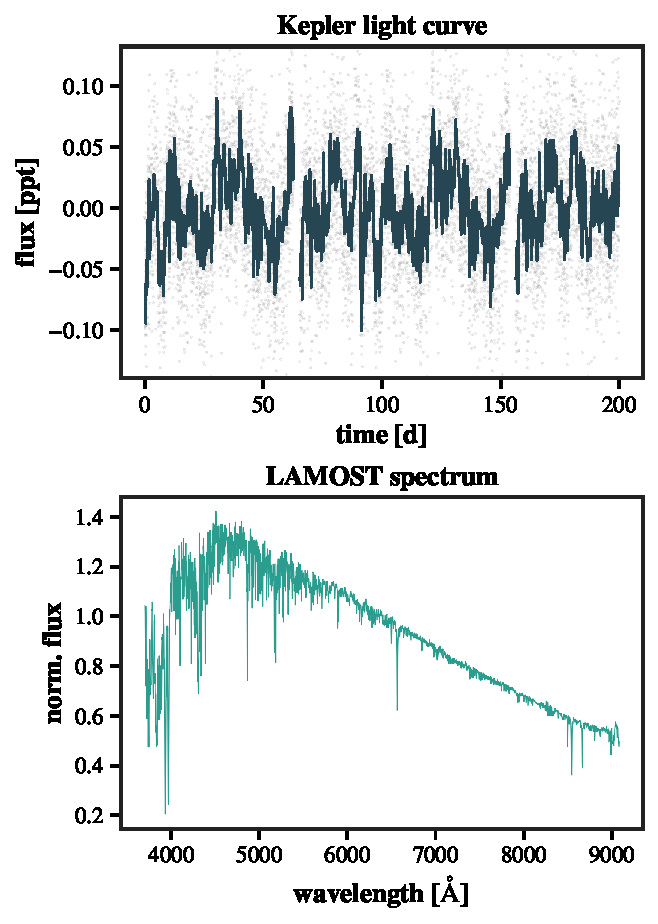
\includegraphics[width=0.31\textwidth]{figs/kic7680114_obs.pdf}};
  \node[lab, anchor=south] at (obs.north) {observations (encoder input)\\[-1pt]};
  % --- catalog record
  \node[anchor=north west] (cat) at ($(obs.north east)+(0.75,0)$) {%
    \begin{tcolorbox}[width=0.225\textwidth, colback=palegrey, colframe=neutral,
        boxrule=0.5pt, arc=1.5pt, left=2pt, right=2pt, top=2pt, bottom=2pt,
        fontupper=\scriptsize]
      \textbf{KIC 7680114}\\[1pt]
      \begin{tabular}{@{}l@{\;}r@{\;}l@{}}
        $T_\mathrm{eff}$ & 5734 K & \dotB \\
        $\log g$ & 4.09 & \\
        $[\mathrm{Fe/H}]$ & $+0.09$ & \dotB \\
        $P_\mathrm{rot}$ & 24.4 d & \dotA \\
        radius & 1.42 $R_\odot$ & \dotA\dotB \\
        mass & 1.10 $M_\odot$ & \\
        age (gyro.) & 6.3 Gyr & \dotA \\
        distance & 170 pc & \dotA \\
        parallax & 5.841 mas & \dotA \\
        $M_K$ & 2.52 & \dotA \\[2pt]
        \multicolumn{2}{@{}l}{dwarf} & \dotA\dotB \\
        \multicolumn{2}{@{}l}{metal-rich quartile} & \dotA\dotB \\
        \multicolumn{2}{@{}l}{not metal-poor} & \dotB \\
        \multicolumn{2}{@{}l}{not Sun-like} & \dotB \\
        \multicolumn{2}{@{}l}{rotation--age mismatch} & \dotA\dotB \\
        \multicolumn{2}{@{}l}{thin disk, $\alpha$-poor} & \dotA \\
      \end{tabular}\\[1pt]
      {\color{neutral}\ldots\ 13 numeric fields + flags}
    \end{tcolorbox}};
  \node[lab, anchor=south] at (cat.north) {catalog record\\[-1pt]};
  % --- two training descriptions
  \node[anchor=north west] (pa) at ($(cat.north east)+(1.0,0)$) {%
    \begin{tcolorbox}[width=0.32\textwidth, colback=white, colframe=teal!80!black,
        boxrule=0.6pt, arc=1.5pt, left=2pt, right=2pt, top=2pt, bottom=2pt,
        fontupper=\scriptsize, title={\dotA\ natural prose}, fonttitle=\scriptsize\bfseries,
        coltitle=deepteal, colbacktitle=paleteal, toptitle=0.5pt, bottomtitle=0.5pt]
      \raggedright
      Catalogued as a main-sequence \hA{dwarf}, the target fits the standard
      parameter ranges. Inferred parameters include a stellar radius of
      \hA{1.42 R\_sun}, a stellar age (derived from gyrochronology) of
      \hA{6.3 $\pm$ 2.2 Gyr}, and a reported distance of \hA{170 pc}. Catalog
      values: absolute K-band magnitude \hA{2.52}; inferred parallax
      \hA{5.841 mas}; photometric rotation period \hA{24.4 d}. Its [Fe/H] sits in
      the \hA{metal-rich} quartile relative to the Kepler field. Its rotation
      period is \hA{inconsistent} with the catalogued age. The target is in the
      \hA{thin-disk} population [\ldots]. It is classified as \hA{alpha-poor} in
      alpha-element abundance.
    \end{tcolorbox}};
  \node[anchor=north west] (pb) at ($(pa.south west)+(0,-0.18)$) {%
    \begin{tcolorbox}[width=0.32\textwidth, colback=white, colframe=coral,
        boxrule=0.6pt, arc=1.5pt, left=2pt, right=2pt, top=2pt, bottom=2pt,
        fontupper=\scriptsize, title={\dotB\ observation log}, fonttitle=\scriptsize\bfseries,
        coltitle=deepteal, colbacktitle=palecoral, toptitle=0.5pt, bottomtitle=0.5pt]
      \raggedright
      Record. \hB{Dwarf.} Fe/H quartile: \hB{metal-rich} ([Fe/H] \hB{0.09}).
      \hB{Above absolute metal-poor cut.} \hB{Rot/age mismatch.}
      \hB{Bulk diverges from Sun.} Teff(spec) \hB{5734 K}. Radius(iso) \hB{1.42 R\_sun}.
    \end{tcolorbox}};
  \node[lab, anchor=south] at (pa.north) {training descriptions (two of six)\\[-1pt]};
  % --- arrows (horizontal, at mid-height of the observation panel)
  \coordinate (ya) at ($(obs.north)!0.45!(obs.south)$);
  \draw[arr] (obs.east |- ya) ++(0.04,0) -- ($(cat.west |- ya)+(-0.04,0)$)
    node[midway, above=2pt, font=\tiny, text=neutral, align=center] {catalog\\pipelines};
  \draw[arr] (cat.east |- ya) ++(0.04,0) -- ($(pa.west |- ya)+(-0.04,0)$)
    node[midway, above=2pt, font=\tiny, text=neutral] {templater};
\end{tikzpicture}
